% Options for packages loaded elsewhere
\PassOptionsToPackage{unicode}{hyperref}
\PassOptionsToPackage{hyphens}{url}
%
\documentclass[
]{article}
\usepackage{amsmath,amssymb}
\usepackage[]{mathpazo}
\usepackage{iftex}
\ifPDFTeX
  \usepackage[T1]{fontenc}
  \usepackage[utf8]{inputenc}
  \usepackage{textcomp} % provide euro and other symbols
\else % if luatex or xetex
  \usepackage{unicode-math}
  \defaultfontfeatures{Scale=MatchLowercase}
  \defaultfontfeatures[\rmfamily]{Ligatures=TeX,Scale=1}
\fi
% Use upquote if available, for straight quotes in verbatim environments
\IfFileExists{upquote.sty}{\usepackage{upquote}}{}
\IfFileExists{microtype.sty}{% use microtype if available
  \usepackage[]{microtype}
  \UseMicrotypeSet[protrusion]{basicmath} % disable protrusion for tt fonts
}{}
\makeatletter
\@ifundefined{KOMAClassName}{% if non-KOMA class
  \IfFileExists{parskip.sty}{%
    \usepackage{parskip}
  }{% else
    \setlength{\parindent}{0pt}
    \setlength{\parskip}{6pt plus 2pt minus 1pt}}
}{% if KOMA class
  \KOMAoptions{parskip=half}}
\makeatother
\usepackage{xcolor}
\usepackage[left=2.5cm,right=2.5cm,top=2cm,bottom=2cm]{geometry}
\usepackage{color}
\usepackage{fancyvrb}
\newcommand{\VerbBar}{|}
\newcommand{\VERB}{\Verb[commandchars=\\\{\}]}
\DefineVerbatimEnvironment{Highlighting}{Verbatim}{commandchars=\\\{\}}
% Add ',fontsize=\small' for more characters per line
\newenvironment{Shaded}{}{}
\newcommand{\AlertTok}[1]{\textcolor[rgb]{1.00,0.00,0.00}{#1}}
\newcommand{\AnnotationTok}[1]{\textcolor[rgb]{0.00,0.50,0.00}{#1}}
\newcommand{\AttributeTok}[1]{#1}
\newcommand{\BaseNTok}[1]{#1}
\newcommand{\BuiltInTok}[1]{#1}
\newcommand{\CharTok}[1]{\textcolor[rgb]{0.00,0.50,0.50}{#1}}
\newcommand{\CommentTok}[1]{\textcolor[rgb]{0.00,0.50,0.00}{#1}}
\newcommand{\CommentVarTok}[1]{\textcolor[rgb]{0.00,0.50,0.00}{#1}}
\newcommand{\ConstantTok}[1]{#1}
\newcommand{\ControlFlowTok}[1]{\textcolor[rgb]{0.00,0.00,1.00}{#1}}
\newcommand{\DataTypeTok}[1]{#1}
\newcommand{\DecValTok}[1]{#1}
\newcommand{\DocumentationTok}[1]{\textcolor[rgb]{0.00,0.50,0.00}{#1}}
\newcommand{\ErrorTok}[1]{\textcolor[rgb]{1.00,0.00,0.00}{\textbf{#1}}}
\newcommand{\ExtensionTok}[1]{#1}
\newcommand{\FloatTok}[1]{#1}
\newcommand{\FunctionTok}[1]{#1}
\newcommand{\ImportTok}[1]{#1}
\newcommand{\InformationTok}[1]{\textcolor[rgb]{0.00,0.50,0.00}{#1}}
\newcommand{\KeywordTok}[1]{\textcolor[rgb]{0.00,0.00,1.00}{#1}}
\newcommand{\NormalTok}[1]{#1}
\newcommand{\OperatorTok}[1]{#1}
\newcommand{\OtherTok}[1]{\textcolor[rgb]{1.00,0.25,0.00}{#1}}
\newcommand{\PreprocessorTok}[1]{\textcolor[rgb]{1.00,0.25,0.00}{#1}}
\newcommand{\RegionMarkerTok}[1]{#1}
\newcommand{\SpecialCharTok}[1]{\textcolor[rgb]{0.00,0.50,0.50}{#1}}
\newcommand{\SpecialStringTok}[1]{\textcolor[rgb]{0.00,0.50,0.50}{#1}}
\newcommand{\StringTok}[1]{\textcolor[rgb]{0.00,0.50,0.50}{#1}}
\newcommand{\VariableTok}[1]{#1}
\newcommand{\VerbatimStringTok}[1]{\textcolor[rgb]{0.00,0.50,0.50}{#1}}
\newcommand{\WarningTok}[1]{\textcolor[rgb]{0.00,0.50,0.00}{\textbf{#1}}}
\usepackage{graphicx}
\makeatletter
\def\maxwidth{\ifdim\Gin@nat@width>\linewidth\linewidth\else\Gin@nat@width\fi}
\def\maxheight{\ifdim\Gin@nat@height>\textheight\textheight\else\Gin@nat@height\fi}
\makeatother
% Scale images if necessary, so that they will not overflow the page
% margins by default, and it is still possible to overwrite the defaults
% using explicit options in \includegraphics[width, height, ...]{}
\setkeys{Gin}{width=\maxwidth,height=\maxheight,keepaspectratio}
% Set default figure placement to htbp
\makeatletter
\def\fps@figure{htbp}
\makeatother
\setlength{\emergencystretch}{3em} % prevent overfull lines
\providecommand{\tightlist}{%
  \setlength{\itemsep}{0pt}\setlength{\parskip}{0pt}}
\setcounter{secnumdepth}{5}
\usepackage{float, graphicx, caption, amssymb, natbib}
\usepackage{amsmath}
\usepackage{listings}
\nocite{*}
\ifLuaTeX
  \usepackage{selnolig}  % disable illegal ligatures
\fi
\IfFileExists{bookmark.sty}{\usepackage{bookmark}}{\usepackage{hyperref}}
\IfFileExists{xurl.sty}{\usepackage{xurl}}{} % add URL line breaks if available
\urlstyle{same} % disable monospaced font for URLs
\hypersetup{
  pdftitle={Imputing Race/Ethnicity Data with Bayesian Improved Surname Geocoding (BISG)},
  hidelinks,
  pdfcreator={LaTeX via pandoc}}

\title{Imputing Race/Ethnicity Data with Bayesian Improved Surname
Geocoding (BISG)}
\usepackage{etoolbox}
\makeatletter
\providecommand{\subtitle}[1]{% add subtitle to \maketitle
  \apptocmd{\@title}{\par {\large #1 \par}}{}{}
}
\makeatother
\subtitle{Description of using the WRU package to Estimate Missing Data}
\author{Eric Moore\footnote{Urban Institute, University of North
  Carolina at Charlotte. Email:
  \href{mailto:emoore99@uncc.edu}{\nolinkurl{emoore99@uncc.edu}}}\\
Kailas Venkitasubramanian\footnote{Urban Institute, University of North
  Carolina at Charlotte. Email:
  \href{mailto:kvenkita@uncc.edu}{\nolinkurl{kvenkita@uncc.edu}}}}
\date{First version: 14 February 2023.\\
This version: 14 March 2023.}

\begin{document}
\maketitle

\vfill

\textbf{Abstract}

This paper provides a detailed walkthrough of how we validated the
estimations of the wru package (R) with the publicly available voter
file in North Carolina. After cleaning the dataset in a way to meet the
standards of wru, we ran the predict race function using the most
recently available 2020 data at the county level. Multiple estimates
were calculated using a combination of the first, middle, and surname
dictionaries. These various predictions are then compared to illustrate
how utilizing all three of these names, even at the county level, can
provide an overall accuracy of 87 percent when predicting an
individual's race/ethnicity. Further examination, however, reveals that
this level of accuracy is not enjoyed by every type of racial/ethnic
group in the dataset.

\newpage

\hypertarget{pre-requisites}{%
\section{Pre-requisites}\label{pre-requisites}}

\hypertarget{files}{%
\subsection{Files}\label{files}}

The statewide voter file for North Carolina represents the only dataset
used for the analysis; this publicly available dataset can be found on
the North Carolina State Board of Elections website and is available
across multiple years and at the county-level.

\hypertarget{requirements}{%
\subsection{Requirements}\label{requirements}}

The following packages are required to run the analysis:

\begin{enumerate}
\def\labelenumi{\arabic{enumi}.}
\tightlist
\item
  tidyverse
\item
  data.table
\item
  wru
\end{enumerate}

Tidyverse includes a host of different packages commonly used for data
management and cleaning. This project relies on dplyr to create the
dataset of interest. Data.table is a package that allows R to import
large datasets more efficiently, specifically for text files, through
the use of the fread command. Finally, we utilize the wru package to
estimate the race/ethnicity of the various individuals within the
dataset.

\hypertarget{creating-the-dataset}{%
\section{Creating the Dataset}\label{creating-the-dataset}}

We begin using the fread function of the data.table package to import
the statewide voter file from North Carolina. Fread presents a viable
alternative to other methods of importing text files due to the size of
the file (approximately 5 million observations).

\begin{Shaded}
\begin{Highlighting}[]
\NormalTok{Undeclared }\OtherTok{\textless{}{-}} \FunctionTok{fread}\NormalTok{(}\StringTok{"\textasciitilde{}/Data/ncvoter\_Statewide.txt"}\NormalTok{)}
\NormalTok{NCcounty }\OtherTok{\textless{}{-}} \FunctionTok{fread}\NormalTok{(}\StringTok{"\textasciitilde{}/Data/Shapefiles/NCDOT\_County\_Boundaries.csv"}\NormalTok{, }
                  \AttributeTok{select=}\FunctionTok{c}\NormalTok{( }\StringTok{"UpperCountyName"}\NormalTok{, }\StringTok{"FIPS"}\NormalTok{))}

\NormalTok{NCcounty}\SpecialCharTok{$}\NormalTok{FIPS }\OtherTok{\textless{}{-}} \FunctionTok{str\_pad}\NormalTok{(NCcounty}\SpecialCharTok{$}\NormalTok{FIPS, }\DecValTok{3}\NormalTok{, }\AttributeTok{pad =} \StringTok{"0"}\NormalTok{)}

\NormalTok{Undeclared }\OtherTok{\textless{}{-}}\NormalTok{ Undeclared }\SpecialCharTok{\%\textgreater{}\%} \FunctionTok{left\_join}\NormalTok{(NCcounty, }
              \AttributeTok{by =} \FunctionTok{c}\NormalTok{( }\StringTok{"county\_desc"} \OtherTok{=} \StringTok{"UpperCountyName"}\NormalTok{) )}
\end{Highlighting}
\end{Shaded}

After successfully bringing in this file and naming it ``Undeclared'',
we then bring in the county-level FIPS information, which will be
important for acquiring the census information later. After creating a
FIPS variable that has the mandatory three spaces for the values, the
final line of code merges these two files together on the county name
(though they are coded differently in the respective datasets) to now
have the information necessary to begin cleaning the dataset.

This begins with the code below:

\begin{Shaded}
\begin{Highlighting}[]
\NormalTok{Undeclared }\OtherTok{\textless{}{-}}\NormalTok{ Undeclared }\SpecialCharTok{\%\textgreater{}\%} 
  \FunctionTok{filter}\NormalTok{(}\SpecialCharTok{!}\NormalTok{( }\FunctionTok{is.na}\NormalTok{(Undeclared}\SpecialCharTok{$}\NormalTok{precinct\_desc ) }\SpecialCharTok{|}\NormalTok{ Undeclared}\SpecialCharTok{$}\NormalTok{precinct\_desc}\SpecialCharTok{==}\StringTok{""}\NormalTok{ ) ) }\SpecialCharTok{\%\textgreater{}\%} 
  \FunctionTok{mutate}\NormalTok{(}\AttributeTok{surname =}\NormalTok{ last\_name, }\AttributeTok{state =} \StringTok{"NC"}\NormalTok{,}
         \AttributeTok{ncpct\_id =} \FunctionTok{as.character}\NormalTok{(precinct\_abbrv),}
         \AttributeTok{sex =} \FunctionTok{ifelse}\NormalTok{(gender\_code }\SpecialCharTok{\%in\%} \StringTok{"F"}\NormalTok{, }\DecValTok{1}\NormalTok{, }\DecValTok{0}\NormalTok{ ),}
         \AttributeTok{PID =} \FunctionTok{ifelse}\NormalTok{(party\_cd }\SpecialCharTok{\%in\%} \StringTok{"DEM"}\NormalTok{, }\DecValTok{1}\NormalTok{,}
                      \FunctionTok{ifelse}\NormalTok{(party\_cd }\SpecialCharTok{\%in\%} \StringTok{"REP"}\NormalTok{, }\DecValTok{2}\NormalTok{, }\DecValTok{0}\NormalTok{)),         }
         \AttributeTok{nc\_re =} \FunctionTok{ifelse}\NormalTok{(race\_code }\SpecialCharTok{\%in\%} \StringTok{"W"} \SpecialCharTok{\&}\NormalTok{ ethnic\_code }\SpecialCharTok{\%ni\%} \StringTok{"HL"}\NormalTok{, }\StringTok{"W"}\NormalTok{,}
                   \FunctionTok{ifelse}\NormalTok{(race\_code }\SpecialCharTok{\%in\%} \StringTok{"B"} \SpecialCharTok{\&}\NormalTok{ ethnic\_code }\SpecialCharTok{\%ni\%} \StringTok{"HL"}\NormalTok{, }\StringTok{"B"}\NormalTok{,}
                   \FunctionTok{ifelse}\NormalTok{(ethnic\_code }\SpecialCharTok{\%in\%} \StringTok{"HL"}\NormalTok{, }\StringTok{"HL"}\NormalTok{,}
                   \FunctionTok{ifelse}\NormalTok{(race\_code }\SpecialCharTok{\%in\%} \StringTok{"A"} \SpecialCharTok{\&}\NormalTok{ ethnic\_code }\SpecialCharTok{\%ni\%} \StringTok{"HL"}\NormalTok{, }\StringTok{"A"}\NormalTok{,}
                   \FunctionTok{ifelse}\NormalTok{(race\_code }\SpecialCharTok{\%ni\%} \FunctionTok{c}\NormalTok{(}\StringTok{"W"}\NormalTok{, }\StringTok{"B"}\NormalTok{, }\StringTok{"A"}\NormalTok{) }\SpecialCharTok{\&} 
\NormalTok{                          ethnic\_code }\SpecialCharTok{\%ni\%} \StringTok{"HL"}\NormalTok{, }\StringTok{"O"}\NormalTok{, }\StringTok{"M"}\NormalTok{))))) )  }\SpecialCharTok{\%\textgreater{}\%} 
\NormalTok{  dplyr}\SpecialCharTok{::}\FunctionTok{select}\NormalTok{(state, }\AttributeTok{county =}\NormalTok{ FIPS, ncpct\_id, ncid, surname, last\_name, }\AttributeTok{first =}\NormalTok{ first\_name, }
                \AttributeTok{middle =}\NormalTok{ middle\_name, nc\_re, race\_code, ethnic\_code)  }\SpecialCharTok{\%\textgreater{}\%} 
  \FunctionTok{distinct}\NormalTok{(ncid, }\AttributeTok{.keep\_all =} \ConstantTok{TRUE}\NormalTok{)}
\end{Highlighting}
\end{Shaded}

As an overview, the preceding code removes any row with missing and/or
empty district (precinct\_desc) values, adds new demographic variables
with modified values, subsets the dataset to only include specific
variables, and finally removes duplicate rows based on the ncid variable
(this is the individual-level identifier provided by the NCSBE). For
more informative purposes, however, we go through and explain the code
in segments.

The row beginning with the filter command removes any row where the
precinct\_desc variable possesses either an NA or an empty string value.
This allows us to remove any observation (registrant) who is not
registered in a recognized district in North Carolina. The mutate
command provides the ability to create several new variables, including:

\begin{itemize}
\tightlist
\item
  A new surname variable with the same values as the last\_name
  variable; in essence, this renames the variable in a way that is in
  line with the requirements of the wru package.
\item
  New geographic identifiers, including a state variable with the value
  ``NC'' and a new ncpct\_id variable with the precinct\_abbrv variable
  converted to character data type.
\item
  For demographic data not related to race/ethnicity, the following
  variables are created, though not included for the analysis:

  \begin{itemize}
  \tightlist
  \item
    A sex variable with values of 1 for ``F'' and 0 for anything else in
    the gender\_code variable.
  \item
    PID (party identification) variable with values of 1 for ``DEM'', 2
    for ``REP'', and 0 for anything else in the party\_cd variable.
  \item
    While these variables are not used in the predictions below, this
    would be the process to make the data in line with the requirements
    of the wru package.
  \end{itemize}
\item
  The nc\_re variable is generated using a series of nested if-else
  statements based on the values of the race\_code and ethnic\_code
  variables. Importantly, we create this new variable to limit
  individuals to having race and ethnicity classifications that are
  exclusive of one another. In other words, we only include White,
  non-Hispanics, non-Hispanic Black/African Americans, etc.
\end{itemize}

The final task in getting the dataset in shape is to remove individuals
without a classification for either race or ethnicity. While normally
this would be our population of interest for imputing data, we want to
eliminate these individuals for the purposes of validating our
predictions later on.

\begin{Shaded}
\begin{Highlighting}[]
\NormalTok{Undeclared.add }\OtherTok{\textless{}{-}}\NormalTok{ Undeclared }\SpecialCharTok{\%\textgreater{}\%} \FunctionTok{filter}\NormalTok{(race\_code }\SpecialCharTok{\%ni\%} \FunctionTok{c}\NormalTok{(}\StringTok{"U"}\NormalTok{, }\StringTok{" "}\NormalTok{) }\SpecialCharTok{\&} 
\NormalTok{                                        ethnic\_code }\SpecialCharTok{\%ni\%} \StringTok{"UN"}\NormalTok{) }\SpecialCharTok{\%\textgreater{}\%} 
\NormalTok{  dplyr}\SpecialCharTok{::}\FunctionTok{select}\NormalTok{(}\SpecialCharTok{{-}}\FunctionTok{c}\NormalTok{(nc\_re, race\_code, ethnic\_code)) }
\end{Highlighting}
\end{Shaded}

The code also removes the race and ethnic variables from the dataset so
the wru prediction can run.

\hypertarget{imputing-raceethnic-data-at-the-individual-level}{%
\section{Imputing Race/Ethnic Data at the
Individual-level}\label{imputing-raceethnic-data-at-the-individual-level}}

\hypertarget{using-the-wru-package-in-r}{%
\subsection{Using the WRU package in
R}\label{using-the-wru-package-in-r}}

Running the BISG model to create the imputed race/ethnic data represents
the next step in the process. We begin by downloading the data at the
geographic unit of interest (here it is the county level in order to
provide a baseline of accuracy for our estimates):

\begin{Shaded}
\begin{Highlighting}[]
\NormalTok{ncCensusData }\OtherTok{\textless{}{-}} \FunctionTok{get\_census\_data}\NormalTok{(}\AttributeTok{key =} \FunctionTok{Sys.getenv}\NormalTok{(}\StringTok{"CENSUS\_API\_KEY"}\NormalTok{),}
                \AttributeTok{states =} \StringTok{"NC"}\NormalTok{, }\AttributeTok{year =} \StringTok{"2020"}\NormalTok{, }\AttributeTok{census.geo =} \StringTok{"county"}\NormalTok{)}
\end{Highlighting}
\end{Shaded}

This code utilizes the get\_census\_data() function with the options to
retrieve Census Bureau data for all North Carolina counties in 2020. The
API key is loaded from an environment variable (footnote here explaining
this process).

We now run the predict\_race() function using the Undeclared.add data
frame and the Census Bureau data to generate the predicted
race/ethnicity for each individual in the data frame:

\begin{Shaded}
\begin{Highlighting}[]
\NormalTok{Undeclared.add }\OtherTok{\textless{}{-}} \FunctionTok{predict\_race}\NormalTok{(}\AttributeTok{voter.file =}\NormalTok{ Undeclared.add, }
                               \AttributeTok{surname.year =} \DecValTok{2020}\NormalTok{,}
                               \AttributeTok{census.geo =} \StringTok{"county"}\NormalTok{, }
                               \AttributeTok{census.data =}\NormalTok{ ncCensusData,}
                               \AttributeTok{year =} \StringTok{"2020"}\NormalTok{,}
                               \AttributeTok{model =} \StringTok{"BISG"}\NormalTok{,}
                               \AttributeTok{names.to.use =} \StringTok{"surname"}\NormalTok{)}
\end{Highlighting}
\end{Shaded}

The options for the model are set as such:

\begin{itemize}
\tightlist
\item
  The census.geo parameter specifies that county-level data should be
  used. The census.data parameter is set to the ncCensusData variable,
  which was created in the previous line.
\item
  The year parameter is set to ``2020'', which matches the year of the
  Census Bureau data.
\item
  The model parameter is set to ``BISG'', which specifies the method
  used for the prediction.
\item
  The names.to.use parameter is set to ``surname'', which indicates that
  only surnames will be used for the prediction.
\end{itemize}

This will provide us with the following predictions:

\hypertarget{translating-the-predictions-into-an-individuals-raceethnicity}{%
\subsection{Translating the predictions into an individuals
``race/ethnicity''}\label{translating-the-predictions-into-an-individuals-raceethnicity}}

While the previous command provides researchers with the predicted
probability of an individual's race/ethnicity across five categories,
the question now becomes what to do with this information? Put another
way, how do we take this information and assign a new predicted value of
race/ethnicity? We answer this with the following code:

\begin{Shaded}
\begin{Highlighting}[]
\NormalTok{Undeclared.add }\OtherTok{\textless{}{-}}\NormalTok{ Undeclared.add }\SpecialCharTok{\%\textgreater{}\%} 
  \FunctionTok{mutate}\NormalTok{(}\AttributeTok{predict\_race =} \FunctionTok{colnames}\NormalTok{(Undeclared.add }\SpecialCharTok{\%\textgreater{}\%} 
\NormalTok{         dplyr}\SpecialCharTok{::}\FunctionTok{select}\NormalTok{(pred.whi}\SpecialCharTok{:}\NormalTok{pred.oth) )[}\FunctionTok{max.col}\NormalTok{(Undeclared.add }\SpecialCharTok{\%\textgreater{}\%} 
\NormalTok{         dplyr}\SpecialCharTok{::}\FunctionTok{select}\NormalTok{(pred.whi}\SpecialCharTok{:}\NormalTok{pred.oth), }\AttributeTok{ties.method =} \StringTok{"random"}\NormalTok{)],}
         \AttributeTok{prace\_new =} \FunctionTok{recode}\NormalTok{(predict\_race, }
                      \StringTok{"pred.whi"} \OtherTok{=} \StringTok{"W"}\NormalTok{,}
                      \StringTok{"pred.bla"} \OtherTok{=} \StringTok{"B"}\NormalTok{,}
                      \StringTok{"pred.his"} \OtherTok{=} \StringTok{"HL"}\NormalTok{,}
                      \StringTok{"pred.asi"} \OtherTok{=} \StringTok{"A"}\NormalTok{,}
                      \StringTok{"pred.oth"} \OtherTok{=} \StringTok{"O"}\NormalTok{)) }\SpecialCharTok{\%\textgreater{}\%}
\NormalTok{  dplyr}\SpecialCharTok{::}\FunctionTok{select}\NormalTok{(ncid, prace\_new)}
\end{Highlighting}
\end{Shaded}

\begin{itemize}
\tightlist
\item
  The mutate() function is used to add two new variables to the data
  frame. Predict\_race is created by selecting the names of the new
  predicted variables (pred.whi through pred.oth) that have the highest
  values for each row.

  \begin{itemize}
  \tightlist
  \item
    This is done using the colnames() and max.col() functions, with
    ties.method = ``random'' to break ties randomly.
  \item
    The resulting variable contains the predicted race for each
    individual.
  \end{itemize}
\item
  Prace\_new is created by using the recode() function to, in essence,
  recode the values based on predict\_race values. The resulting
  variable contains the predicted race for each row in a format
  consistent with the previous code example.
\item
  The dataset is then limited to only the ncid and prace\_new variables.
\end{itemize}

\hypertarget{validating-the-predictions-from-wru}{%
\subsection{Validating the predictions from
WRU}\label{validating-the-predictions-from-wru}}

The final step in the process is to check whether the predictions of the
BISG model matches with the self-reported race/ethnicity of registered
voters in North Carolina. To do this, we need to filter out any rows
with missing or unknown data related to race or ethnicity before joining
the original dataset with the new dataframe containing the predicted
race/ethnicity.

These two data frames are merged using the unique identifier for each
voter:

\begin{Shaded}
\begin{Highlighting}[]
\NormalTok{Undeclared }\OtherTok{\textless{}{-}}\NormalTok{ Undeclared }\SpecialCharTok{\%\textgreater{}\%} \FunctionTok{filter}\NormalTok{(race\_code }\SpecialCharTok{\%ni\%} \FunctionTok{c}\NormalTok{(}\StringTok{"U"}\NormalTok{, }\StringTok{" "}\NormalTok{) }\SpecialCharTok{\&}\NormalTok{ ethnic\_code }\SpecialCharTok{\%ni\%} \StringTok{"UN"}\NormalTok{) }\SpecialCharTok{\%\textgreater{}\%}
  \FunctionTok{left\_join}\NormalTok{(Undeclared.add, }\AttributeTok{by =} \StringTok{"ncid"}\NormalTok{ )}
\end{Highlighting}
\end{Shaded}

The resulting dataframe can now be used to determine the level of
accuracy for the BISG predictions when it comes to the race/ethnicity of
registered voters in North Carolina. To perform this validation, we run
the final chunk of code:

\begin{Shaded}
\begin{Highlighting}[]
\NormalTok{Undeclared }\OtherTok{\textless{}{-}}\NormalTok{  Undeclared }\SpecialCharTok{\%\textgreater{}\%} \FunctionTok{filter}\NormalTok{(nc\_re }\SpecialCharTok{\%ni\%} \StringTok{"M"}\NormalTok{) }\SpecialCharTok{\%\textgreater{}\%} 
  \FunctionTok{mutate}\NormalTok{(}\AttributeTok{Race\_sur =} \FunctionTok{ifelse}\NormalTok{(nc\_re }\SpecialCharTok{\%in\%} \StringTok{"W"} \SpecialCharTok{\&}\NormalTok{ prace\_new }\SpecialCharTok{\%in\%} \StringTok{"W"}\NormalTok{, }\DecValTok{1}\NormalTok{, }
                    \FunctionTok{ifelse}\NormalTok{(nc\_re }\SpecialCharTok{\%in\%} \StringTok{"B"} \SpecialCharTok{\&}\NormalTok{ prace\_new }\SpecialCharTok{\%in\%} \StringTok{"B"}\NormalTok{, }\DecValTok{1}\NormalTok{, }
                    \FunctionTok{ifelse}\NormalTok{(nc\_re }\SpecialCharTok{\%in\%} \StringTok{"A"} \SpecialCharTok{\&}\NormalTok{ prace\_new }\SpecialCharTok{\%in\%} \StringTok{"A"}\NormalTok{, }\DecValTok{1}\NormalTok{,}
                    \FunctionTok{ifelse}\NormalTok{(nc\_re }\SpecialCharTok{\%in\%} \StringTok{"O"} \SpecialCharTok{\&}\NormalTok{ prace\_new }\SpecialCharTok{\%in\%} \StringTok{"O"}\NormalTok{, }\DecValTok{1}\NormalTok{,}
                    \FunctionTok{ifelse}\NormalTok{(nc\_re }\SpecialCharTok{\%in\%} \StringTok{"HL"} \SpecialCharTok{\&}\NormalTok{ prace\_new }\SpecialCharTok{\%in\%} \StringTok{"HL"}\NormalTok{, }\DecValTok{1}\NormalTok{, }\DecValTok{0}\NormalTok{)))))) }\SpecialCharTok{\%\textgreater{}\%} 
\NormalTok{  dplyr}\SpecialCharTok{::}\FunctionTok{select}\NormalTok{(}\SpecialCharTok{{-}}\FunctionTok{c}\NormalTok{(prace\_new)) }

\NormalTok{check }\OtherTok{\textless{}{-}} \FunctionTok{table}\NormalTok{(Undeclared}\SpecialCharTok{$}\NormalTok{Race\_sur) }
\NormalTok{check }\SpecialCharTok{/} \FunctionTok{sum}\NormalTok{(check) }
\FunctionTok{rm}\NormalTok{(check)}
\end{Highlighting}
\end{Shaded}

After filtering any rows where the race is listed as ``Multiracial'', We
then create a new variable indicating whether the race listed in the
original dataset matches the predicted race based on surname. If the
original race matches the predicted race, the value of this variable is
set to 1, and it is set to 0 otherwise. The final lines of code
calculates the proportion of voters whose original and predicted race
match and outputs this as a table.

\hypertarget{results}{%
\section{Results}\label{results}}

In order to provide an accurate assessment of the BISG model, I
performed three separate predictions that utilized the three different
options for names: surname (last name) only, surname and first name, and
surname, first, and middle name. The predictions were then compared to
the self-reported race/ethnicity of the respective registrant. All of
these predictions utilized Census data at the county level, though there
is a possibility of utilizing lower geographical units such as the
Census Tract, Block Group, or even Block if desired. The results of the
various BISG predictions and their accuracy to the self-reported
identity of Whites, Blacks/African Americans, Hispanic/Latinos, and
Asians is reported below.

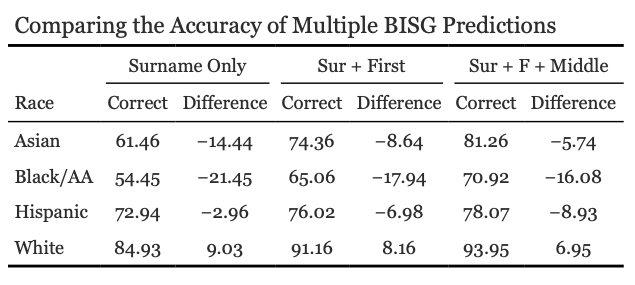
\includegraphics[width=0.7\textwidth,height=\textheight]{tab1.png}

All else being equal, we see an increase of approximately 11 percent
accuracy going from using surname (last names) exclusively to using the
first, middle, and surname in the predictive model (76 percent predicted
correctly compared to 87 percent predicted correctly, respectively). The
issue, however, is that the accuracy of the model appears to be biased
toward whites. In every model, whites are the only group that
consistently outperform the mean accuracy of the model while
Blacks/African Americans perform the worst. While this bias is reduced
as we utilize more information in the prediction, and the overall
accuracy of the model is something that provides promise for research,
this underestimation of minority groups proposes a significant drawback,
particularly for community research.

\end{document}
